\documentclass[border=4mm]{standalone}
\usepackage[T1]{fontenc}
\usepackage{helvet}
\renewcommand{\familydefault}{\sfdefault}
\usepackage{tikz}
\usepackage{amsmath,amssymb}
\usetikzlibrary{calc,positioning,arrows.meta,shadows.blur,fit,shapes.geometric,
                 decorations.pathmorphing}

% PALETTE
\definecolor{L1}{HTML}{0D47A1}
\definecolor{L1bg}{HTML}{E3F2FD}
\definecolor{L2}{HTML}{00695C}
\definecolor{L2bg}{HTML}{E0F2F1}
\definecolor{L3}{HTML}{E65100}
\definecolor{L3bg}{HTML}{FFF3E0}
\definecolor{L4}{HTML}{6A1B9A}
\definecolor{L4bg}{HTML}{F3E5F5}
\definecolor{gold}{HTML}{F9A825}
\definecolor{dk}{HTML}{212121}
\definecolor{mg}{HTML}{616161}
\definecolor{ac}{HTML}{37474F}
\definecolor{sg}{HTML}{2E7D32}
\definecolor{wr}{HTML}{C62828}

\tikzset{
  layer/.style={rounded corners=10pt, draw=#1, line width=2pt, fill=#1!8, inner sep=0pt},
  badge/.style={circle, minimum size=30pt, font=\bfseries\Large\sffamily, fill=#1, text=white, inner sep=0pt,
    blur shadow={shadow blur steps=4, shadow xshift=1pt, shadow yshift=-1pt, shadow opacity=30}},
  ltitle/.style={font=\bfseries\LARGE\sffamily, text=#1},
  lsub/.style={font=\large\sffamily, text=#1!70!black},
  keyeq/.style={rounded corners=6pt, draw=#1, line width=1.2pt, fill=white, inner sep=10pt,
    blur shadow={shadow blur steps=3, shadow xshift=0.5pt, shadow yshift=-0.5pt, shadow opacity=20}},
  pill/.style={rounded corners=12pt, draw=#1!60!black, line width=0.8pt, fill=#1!15, inner sep=8pt,
    font=\normalsize\sffamily, text=dk, minimum height=28pt},
  bigarrow/.style={-{Triangle[length=10pt,width=8pt]}, line width=3.5pt, ac},
  gtside/.style={-{Triangle[length=8pt,width=6pt]}, line width=2.5pt, gold, dashed, dash pattern=on 6pt off 4pt},
  cnode/.style={circle, minimum size=24pt, font=\bfseries\small\sffamily, fill=#1!20, draw=#1, line width=1.2pt, inner sep=0pt},
}

\begin{document}
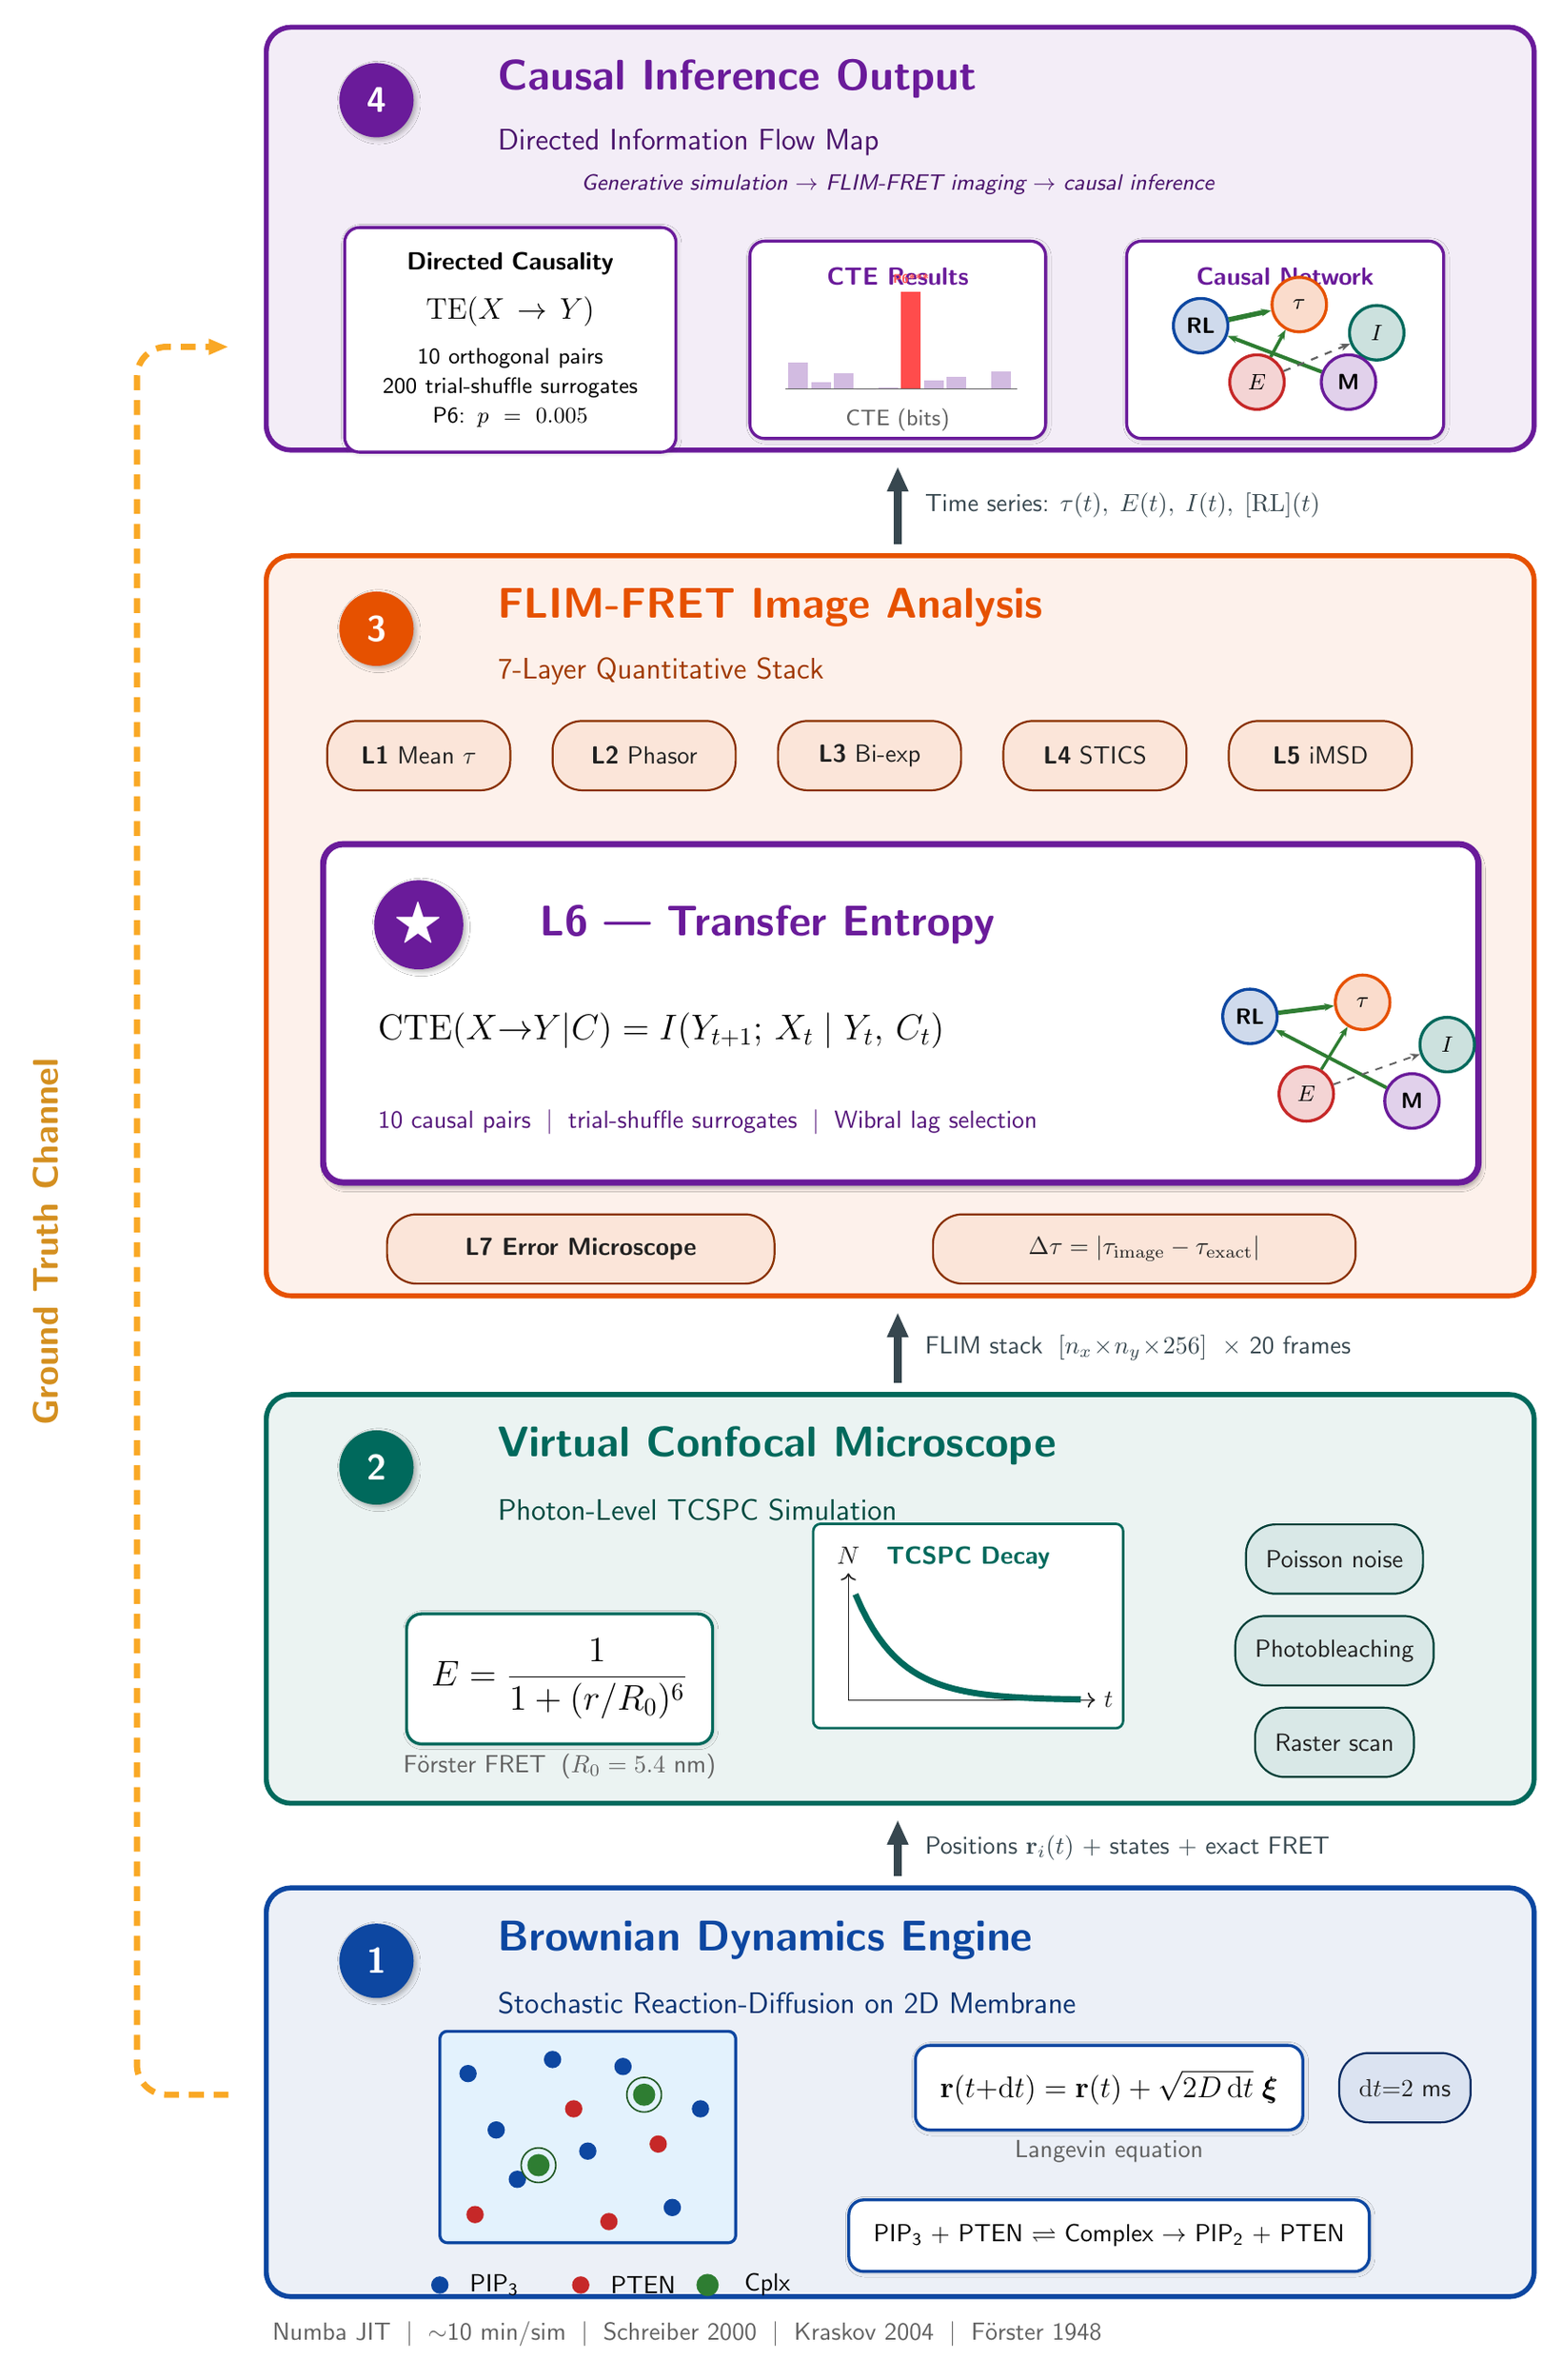
\begin{tikzpicture}[x=1cm, y=1cm]

\def\W{18}
\def\C{9}

% Layer positions and heights
\def\Ya{0}     \def\Ha{5.8}
\def\Yb{7.0}   \def\Hb{5.8}
\def\Yc{14.2}  \def\Hc{10.5}
\def\Yd{26.2}  \def\Hd{6.0}

% ================================================================
% LAYER 1 — BROWNIAN DYNAMICS
% ================================================================
\node[layer=L1, minimum width=\W cm, minimum height=\Ha cm, anchor=south west] (C1) at (0,\Ya) {};

\node[badge=L1] at (1.6, \Ya+\Ha-1.0) {\textsf{1}};
\node[ltitle=L1, anchor=west] at (3.2, \Ya+\Ha-0.7) {Brownian Dynamics Engine};
\node[lsub=L1, anchor=west] at (3.2, \Ya+\Ha-1.6) {Stochastic Reaction-Diffusion on 2D Membrane};

% Membrane schematic
\begin{scope}[shift={(2.5, \Ya+0.8)}]
  \draw[L1, line width=1.2pt, rounded corners=3pt, fill=L1bg] (0,0) rectangle (4.2,3.0);
  \foreach \x/\y in {0.4/2.4, 1.1/0.9, 2.6/2.5, 3.3/0.5, 3.7/1.9, 0.8/1.6, 2.1/1.3, 1.6/2.6} {
    \fill[L1] (\x,\y) circle (3.5pt); }
  \foreach \x/\y in {0.5/0.4, 1.9/1.9, 3.1/1.4, 2.4/0.3} {
    \fill[wr] (\x,\y) circle (3.5pt); }
  \foreach \x/\y in {1.4/1.1, 2.9/2.1} {
    \fill[sg] (\x,\y) circle (4.5pt);
    \draw[sg!70!black, line width=0.6pt] (\x,\y) circle (7pt); }
  % Legend
  \fill[L1] (0.0,-0.6) circle (3.5pt);
  \node[font=\normalsize\sffamily, anchor=west] at (0.3,-0.6) {PIP\textsubscript{3}};
  \fill[wr] (2.0,-0.6) circle (3.5pt);
  \node[font=\normalsize\sffamily, anchor=west] at (2.3,-0.6) {PTEN};
  \fill[sg] (3.8,-0.6) circle (4.5pt);
  \node[font=\normalsize\sffamily, anchor=west] at (4.2,-0.6) {Cplx};
\end{scope}

% Langevin equation
\node[keyeq=L1, font=\large] (eq1) at (12.0, \Ya+3.0)
  {$\mathbf{r}(t{+}\mathrm{d}t) = \mathbf{r}(t) + \sqrt{2D\,\mathrm{d}t}\;\boldsymbol{\xi}$};
\node[font=\normalsize\sffamily, text=mg, anchor=north] at (eq1.south) {Langevin equation};

% Reaction
\node[keyeq=L1, font=\normalsize] at (12.0, \Ya+0.9)
  {PIP\textsubscript{3} + PTEN $\rightleftharpoons$ Complex $\to$ PIP\textsubscript{2} + PTEN};

\node[pill=L1] at (16.2, \Ya+3.0) {$\mathrm{d}t{=}2$ ms};

% ================================================================
% ARROW 1 → 2
% ================================================================
\draw[bigarrow] (\C, \Ya+\Ha+0.2) -- (\C, \Yb-0.2)
  node[midway, right=6pt, font=\normalsize\sffamily, text=ac]
  {Positions $\mathbf{r}_i(t)$ + states + exact FRET};

% ================================================================
% LAYER 2 — VIRTUAL MICROSCOPE
% ================================================================
\node[layer=L2, minimum width=\W cm, minimum height=\Hb cm, anchor=south west] (C2) at (0,\Yb) {};

\node[badge=L2] at (1.6, \Yb+\Hb-1.0) {\textsf{2}};
\node[ltitle=L2, anchor=west] at (3.2, \Yb+\Hb-0.7) {Virtual Confocal Microscope};
\node[lsub=L2, anchor=west] at (3.2, \Yb+\Hb-1.6) {Photon-Level TCSPC Simulation};

% FRET equation
\node[keyeq=L2, font=\Large] (eqf) at (4.2, \Yb+1.8)
  {$E = \dfrac{1}{1 + (r/R_0)^6}$};
\node[font=\normalsize\sffamily, text=mg, anchor=north] at (eqf.south)
  {F\"orster FRET \;($R_0 = 5.4$ nm)};

% TCSPC curve
\begin{scope}[shift={(10.0, \Yb+1.5)}]
  \draw[L2, line width=1pt, rounded corners=3pt, fill=white] (-2.2,-0.4) rectangle (2.2,2.5);
  \node[font=\normalsize\sffamily\bfseries, text=L2, anchor=north] at (0,2.3) {TCSPC Decay};
  \draw[dk, line width=0.6pt, ->] (-1.7,0) -- (1.8,0) node[right, font=\normalsize] {$t$};
  \draw[dk, line width=0.6pt, ->] (-1.7,0) -- (-1.7,1.8) node[above, font=\normalsize] {$N$};
  \draw[L2, line width=2.5pt, domain=-1.6:1.6, samples=40]
    plot (\x, {1.5*exp(-1.6*(\x+1.6))});
\end{scope}

% Noise pills
\node[pill=L2] at (15.2, \Yb+3.5) {Poisson noise};
\node[pill=L2] at (15.2, \Yb+2.2) {Photobleaching};
\node[pill=L2] at (15.2, \Yb+0.9) {Raster scan};

% ================================================================
% ARROW 2 → 3
% ================================================================
\draw[bigarrow] (\C, \Yb+\Hb+0.2) -- (\C, \Yc-0.2)
  node[midway, right=6pt, font=\normalsize\sffamily, text=ac]
  {FLIM stack \;$[n_x \!\times\! n_y \!\times\! 256]$ \;$\times$ 20 frames};

% ================================================================
% LAYER 3 — FLIM-FRET ANALYSIS
% ================================================================
\node[layer=L3, minimum width=\W cm, minimum height=\Hc cm, anchor=south west] (C3) at (0,\Yc) {};

\node[badge=L3] at (1.6, \Yc+\Hc-1.0) {\textsf{3}};
\node[ltitle=L3, anchor=west] at (3.2, \Yc+\Hc-0.7) {FLIM-FRET Image Analysis};
\node[lsub=L3, anchor=west] at (3.2, \Yc+\Hc-1.6) {7-Layer Quantitative Stack};

% L1-L5 pills row
\pgfmathsetmacro{\pillY}{\Yc+\Hc-2.8}
\node[pill=L3, minimum width=2.6cm] at (2.2, \pillY) {\textbf{L1} Mean $\tau$};
\node[pill=L3, minimum width=2.6cm] at (5.4, \pillY) {\textbf{L2} Phasor};
\node[pill=L3, minimum width=2.6cm] at (8.6, \pillY) {\textbf{L3} Bi-exp};
\node[pill=L3, minimum width=2.6cm] at (11.8, \pillY) {\textbf{L4} STICS};
\node[pill=L3, minimum width=2.6cm] at (15.0, \pillY) {\textbf{L5} iMSD};

% L6 TRANSFER ENTROPY — THE STAR
\node[rounded corners=8pt, draw=L4, line width=2.5pt, fill=white,
      minimum width=16.4cm, minimum height=4.8cm,
      blur shadow={shadow blur steps=6, shadow xshift=1pt, shadow yshift=-2pt, shadow opacity=35},
      anchor=south west] (TEbox) at (0.8, \Yc+1.6) {};

% Star badge
\node[badge=L4, minimum size=36pt, font=\bfseries\huge] at (2.2, \Yc+5.3) {$\bigstar$};

% Title
\node[font=\bfseries\LARGE\sffamily, text=L4, anchor=west] at (3.8, \Yc+5.3)
  {L6 --- Transfer Entropy};

% THE equation — BIG
\node[font=\Large, anchor=west] at (1.5, \Yc+3.8)
  {$\mathrm{CTE}(X{\to}Y|C) = I(Y_{t+1};\,X_t\;|\;Y_t,\,C_t)$};

% Info line
\node[font=\normalsize\sffamily, text=L4!80!black, anchor=west] at (1.5, \Yc+2.5)
  {10 causal pairs \;\textbar\; trial-shuffle surrogates \;\textbar\; Wibral lag selection};

% Mini causal network
\begin{scope}[shift={(14.8, \Yc+3.2)}]
  \node[cnode=L1, minimum size=22pt] (cRL) at (-0.8, 0.8) {RL};
  \node[cnode=L3, minimum size=22pt] (ctau) at (0.8, 1.0) {$\tau$};
  \node[cnode=L2, minimum size=22pt] (cI) at (2.0, 0.4) {$I$};
  \node[cnode=wr, minimum size=22pt] (cE) at (0.0, -0.3) {$E$};
  \node[cnode=L4, minimum size=22pt] (cM) at (1.5, -0.4) {M};
  \draw[-{Stealth[length=4pt]}, sg, line width=1.8pt] (cRL) -- (ctau);
  \draw[-{Stealth[length=4pt]}, sg, line width=1.4pt] (cM) -- (cRL);
  \draw[-{Stealth[length=4pt]}, sg, line width=1.2pt] (cE) -- (ctau);
  \draw[-{Stealth[length=4pt]}, mg, line width=0.7pt, dashed] (cE) -- (cI);
\end{scope}

% L7 Error Microscope
\node[pill=L3, minimum width=5.5cm, font=\normalsize\sffamily\bfseries] at (4.5, \Yc+0.7)
  {\textbf{L7} Error Microscope};
\node[pill=L3, minimum width=6cm] at (12.5, \Yc+0.7)
  {$\Delta\tau = |\tau_\mathrm{image} - \tau_\mathrm{exact}|$};

% ================================================================
% ARROW 3 → 4
% ================================================================
\draw[bigarrow] (\C, \Yc+\Hc+0.2) -- (\C, \Yd-0.2)
  node[midway, right=6pt, font=\normalsize\sffamily, text=ac]
  {Time series: $\tau(t),\; E(t),\; I(t),\; [\mathrm{RL}](t)$};

% ================================================================
% LAYER 4 — CAUSAL INFERENCE OUTPUT
% ================================================================
\node[layer=L4, minimum width=\W cm, minimum height=\Hd cm, anchor=south west] (C4) at (0,\Yd) {};

\node[badge=L4] at (1.6, \Yd+\Hd-1.0) {\textsf{4}};
\node[ltitle=L4, anchor=west] at (3.2, \Yd+\Hd-0.7) {Causal Inference Output};
\node[lsub=L4, anchor=west] at (3.2, \Yd+\Hd-1.6) {Directed Information Flow Map};

% Tagline — subtle, not dominant
\node[font=\small\sffamily\itshape, text=L4!70!black]
  at (\C, \Yd+3.8)
  {Generative simulation $\to$ FLIM-FRET imaging $\to$ causal inference};

% TE concept — compact, no specific data
\begin{scope}[shift={(3.5, \Yd+1.6)}]
  \node[keyeq=L4, text width=4.0cm, align=center, minimum height=2.8cm] at (0,0) {%
    {\bfseries\normalsize Directed Causality}\\[8pt]
    {\large $\mathrm{TE}(X \!\to\! Y)$}\\[6pt]
    {\small 10 orthogonal pairs}\\
    {\small 200 trial-shuffle surrogates}\\
    {\small P6: $p = 0.005$}
  };
\end{scope}

% CTE Bar Chart (10 pairs)
\begin{scope}[shift={(9.0, \Yd+1.6)}]
  \node[keyeq=L4, minimum width=4.2cm, minimum height=2.8cm] at (0,0) {};
  \node[font=\normalsize\sffamily\bfseries, text=L4, anchor=north] at (0,1.15) {CTE Results};
  % Bar chart: 10 bars, P6 highlighted
  \foreach \i/\h/\c in {0/0.15/L4!30, 1/0.04/L4!30, 2/0.09/L4!30, 3/0.00/L4!30, 4/0.01/L4!30, 5/0.55/red!70, 6/0.05/L4!30, 7/0.07/L4!30, 8/0.00/L4!30, 9/0.10/L4!30} {
    \fill[\c] (-1.55+\i*0.32, -0.7) rectangle (-1.55+\i*0.32+0.28, -0.7+\h*2.5);
  }
  % Axis
  \draw[mg, thin] (-1.6, -0.7) -- (1.7, -0.7);
  % P6 label
  \node[font=\tiny\sffamily\bfseries, text=red!70, anchor=south] at (-1.55+5*0.32+0.14, -0.7+0.55*2.5) {P6***};
  \node[font=\small\sffamily, text=mg, anchor=north] at (0,-0.85) {CTE (bits)};
\end{scope}

% Causal Network
\begin{scope}[shift={(14.5, \Yd+1.6)}]
  \node[keyeq=L4, minimum width=4.5cm, minimum height=2.8cm] at (0,0) {};
  \node[font=\normalsize\sffamily\bfseries, text=L4, anchor=north] at (0,1.15) {Causal Network};
  \node[cnode=L1, minimum size=22pt] (n1) at (-1.2, 0.2) {RL};
  \node[cnode=L3, minimum size=22pt] (n2) at (0.2, 0.5) {$\tau$};
  \node[cnode=L2, minimum size=22pt] (n3) at (1.3, 0.1) {$I$};
  \node[cnode=wr, minimum size=22pt] (n4) at (-0.4, -0.6) {$E$};
  \node[cnode=L4, minimum size=22pt] (n5) at (0.9, -0.6) {M};
  \draw[-{Stealth[length=4pt]}, sg, line width=2pt] (n1) -- (n2);
  \draw[-{Stealth[length=4pt]}, sg, line width=1.5pt] (n5) -- (n1);
  \draw[-{Stealth[length=4pt]}, sg, line width=1.3pt] (n4) -- (n2);
  \draw[-{Stealth[length=4pt]}, mg, line width=0.8pt, dashed] (n4) -- (n3);
\end{scope}

% ================================================================
% GROUND TRUTH BYPASS
% ================================================================
\draw[gtside, rounded corners=12pt]
  (-0.5, \Ya+\Ha*0.5) -- (-1.8, \Ya+\Ha*0.5)
  -- (-1.8, \Yd+1.5) -- (-0.5, \Yd+1.5);
\node[rotate=90, font=\Large\sffamily\bfseries, text=gold!85!black, anchor=south]
  at (-2.8, 15) {Ground Truth Channel};

% ================================================================
% HEADER + FOOTER
% ================================================================
% Title removed for Nature Communications format (caption in text)

\node[font=\normalsize\sffamily, text=mg, anchor=south west]
  at (0, \Ya-0.8)
  {Numba JIT \;\textbar\; ${\sim}$10 min/sim \;\textbar\;
  Schreiber 2000 \;\textbar\; Kraskov 2004 \;\textbar\; F\"orster 1948};

\end{tikzpicture}
\end{document}
